% ============================================================
% DIAGRAM: Perceptron Architecture (1958)
% ============================================================
% Caption: Figure 2.1: The Perceptron architecture.
%          (Adapted from Rosenblatt, 1958, p. 387)
% ============================================================

\documentclass[tikz,border=10pt]{standalone}
\usepackage{tikz}
\usepackage{amsmath}
\usepackage{amsfonts}

\usetikzlibrary{shapes,arrows,positioning,fit,calc,backgrounds}

\begin{document}

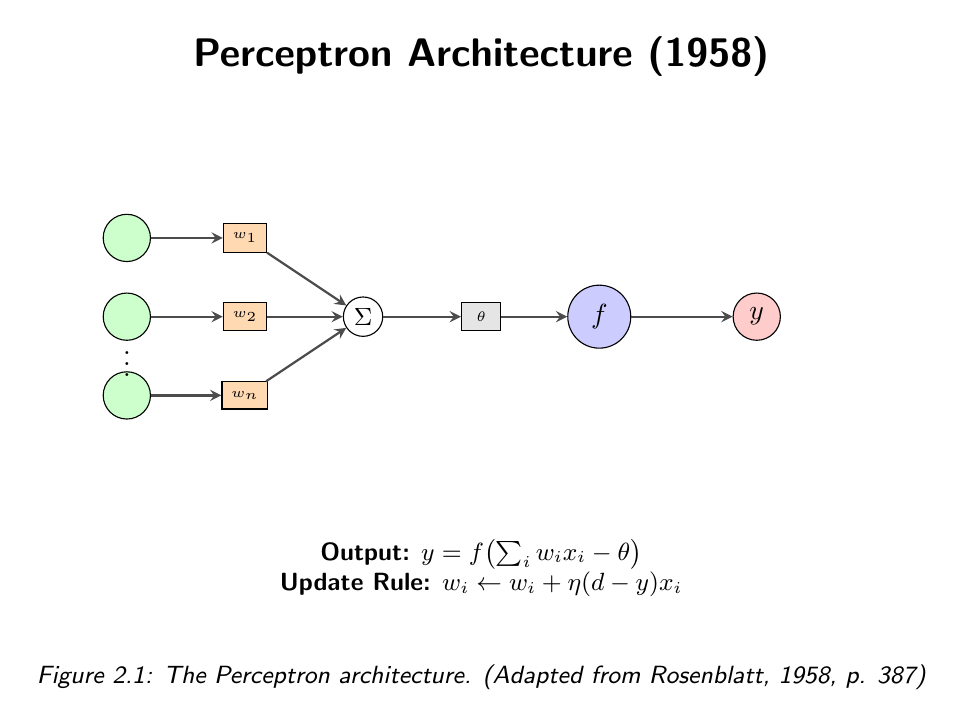
\begin{tikzpicture}[
    input/.style={draw, circle, minimum size=0.6cm, inner sep=0pt, fill=green!20},
    weight/.style={draw, rectangle, minimum width=0.5cm, minimum height=0.3cm, fill=orange!30, font=\tiny},
    sum/.style={draw, circle, minimum size=0.5cm, inner sep=0pt, fill=white, font=\sffamily\small},
    neuron/.style={draw, circle, minimum size=0.8cm, inner sep=0pt, fill=blue!20},
    output/.style={draw, circle, minimum size=0.6cm, inner sep=0pt, fill=red!20},
    label/.style={font=\sffamily\small},
    title/.style={font=\sffamily\Large\bfseries},
    caption/.style={font=\sffamily\small\itshape},
    edge/.style={-stealth, thick, draw=black!70},
]

\node[title] at (0, 3.8) {Perceptron Architecture (1958)};

% Input layer
\node[input] (x1) at (-4.5, 1.5) {};
\node[input] (x2) at (-4.5, 0.5) {};
\node[input] (xn) at (-4.5, -0.5) {};
\node at (-4.5, 0) {$\vdots$};

% Weights
\node[weight] (w1) at (-3, 1.5) {$w_1$};
\node[weight] (w2) at (-3, 0.5) {$w_2$};
\node[weight] (wn) at (-3, -0.5) {$w_n$};

% Sum
\node[sum] (sum) at (-1.5, 0.5) {$\Sigma$};

% Threshold
\node[weight, fill=gray!20] (theta) at (0, 0.5) {$\theta$};

% Neuron
\node[neuron] (neuron) at (1.5, 0.5) {$f$};

% Output
\node[output] (y) at (3.5, 0.5) {$y$};

% Edges
\draw[edge] (x1) -- (w1);
\draw[edge] (x2) -- (w2);
\draw[edge] (xn) -- (wn);
\draw[edge] (w1) -- (sum);
\draw[edge] (w2) -- (sum);
\draw[edge] (wn) -- (sum);
\draw[edge] (sum) -- (theta);
\draw[edge] (theta) -- (neuron);
\draw[edge] (neuron) -- (y);

% Equation
\node[align=center, font=\sffamily\small, anchor=north] at (0, -2.2) {
  \textbf{Output:} $y = f\!\left( \sum_i w_i x_i - \theta \right)$ \\
  \textbf{Update Rule:} $w_i \leftarrow w_i + \eta (d - y) x_i$
};

\node[caption, anchor=north] at (0, -3.8) {
  Figure 2.1: The Perceptron architecture. (Adapted from Rosenblatt, 1958, p. 387)
};

\end{tikzpicture}
\end{document}
